\documentclass[a4paper]{article}

%% Language and font encodings
\usepackage[english]{babel}
\usepackage[utf8x]{inputenc}
\usepackage[T1]{fontenc}

%% Sets page size and margins
\usepackage[a4paper,top=3cm,bottom=2cm,left=3cm,right=3cm,marginparwidth=1.75cm]{geometry}

%% Useful packages
\usepackage{amsmath}
\usepackage{graphicx}
\usepackage{mathtools}
\usepackage[colorinlistoftodos]{todonotes}
\usepackage[colorlinks=true, allcolors=blue]{hyperref}

\title{Training a Neural Network - A Numerical Example}
\author{Raphael B. Alampay}

\begin{document}
\maketitle

\begin{abstract}
Neural networks are powerful function approximation tools. In the case of pattern recognition, we use neural networks to approximate a discriminative function for classification in a supervised learning fashion. This paper takes a look at a quantitative approach in training a neural network given actual numerical examples. This will allow the student to understand each step of the training process.
\end{abstract}

\section{Introduction}
Neural networks are biologically inspired computational models that attempts to solve classification problems. It is composed on \textbf{neurons} which holds and processes values in the network. You can think of these values as signal strengths that aim to mimic how chemical reactions occur in the brain. The higher the value, the stronger the signal. In biology, neurons transmit and receive signals to and from other neurons by means of dendrites. These propagations are modelled in the neural network by means of weight values. Since a neuron may receive values from more than one neuron, it accounts all these weight value connections before attempting to fire a signal thus simulating how we "react" to certain stimuli. Training the neural network simply means adjusting these weights based on what we already know in order for the model to properly "react" to a certain input.

\begin{figure}[!htb]
\centering
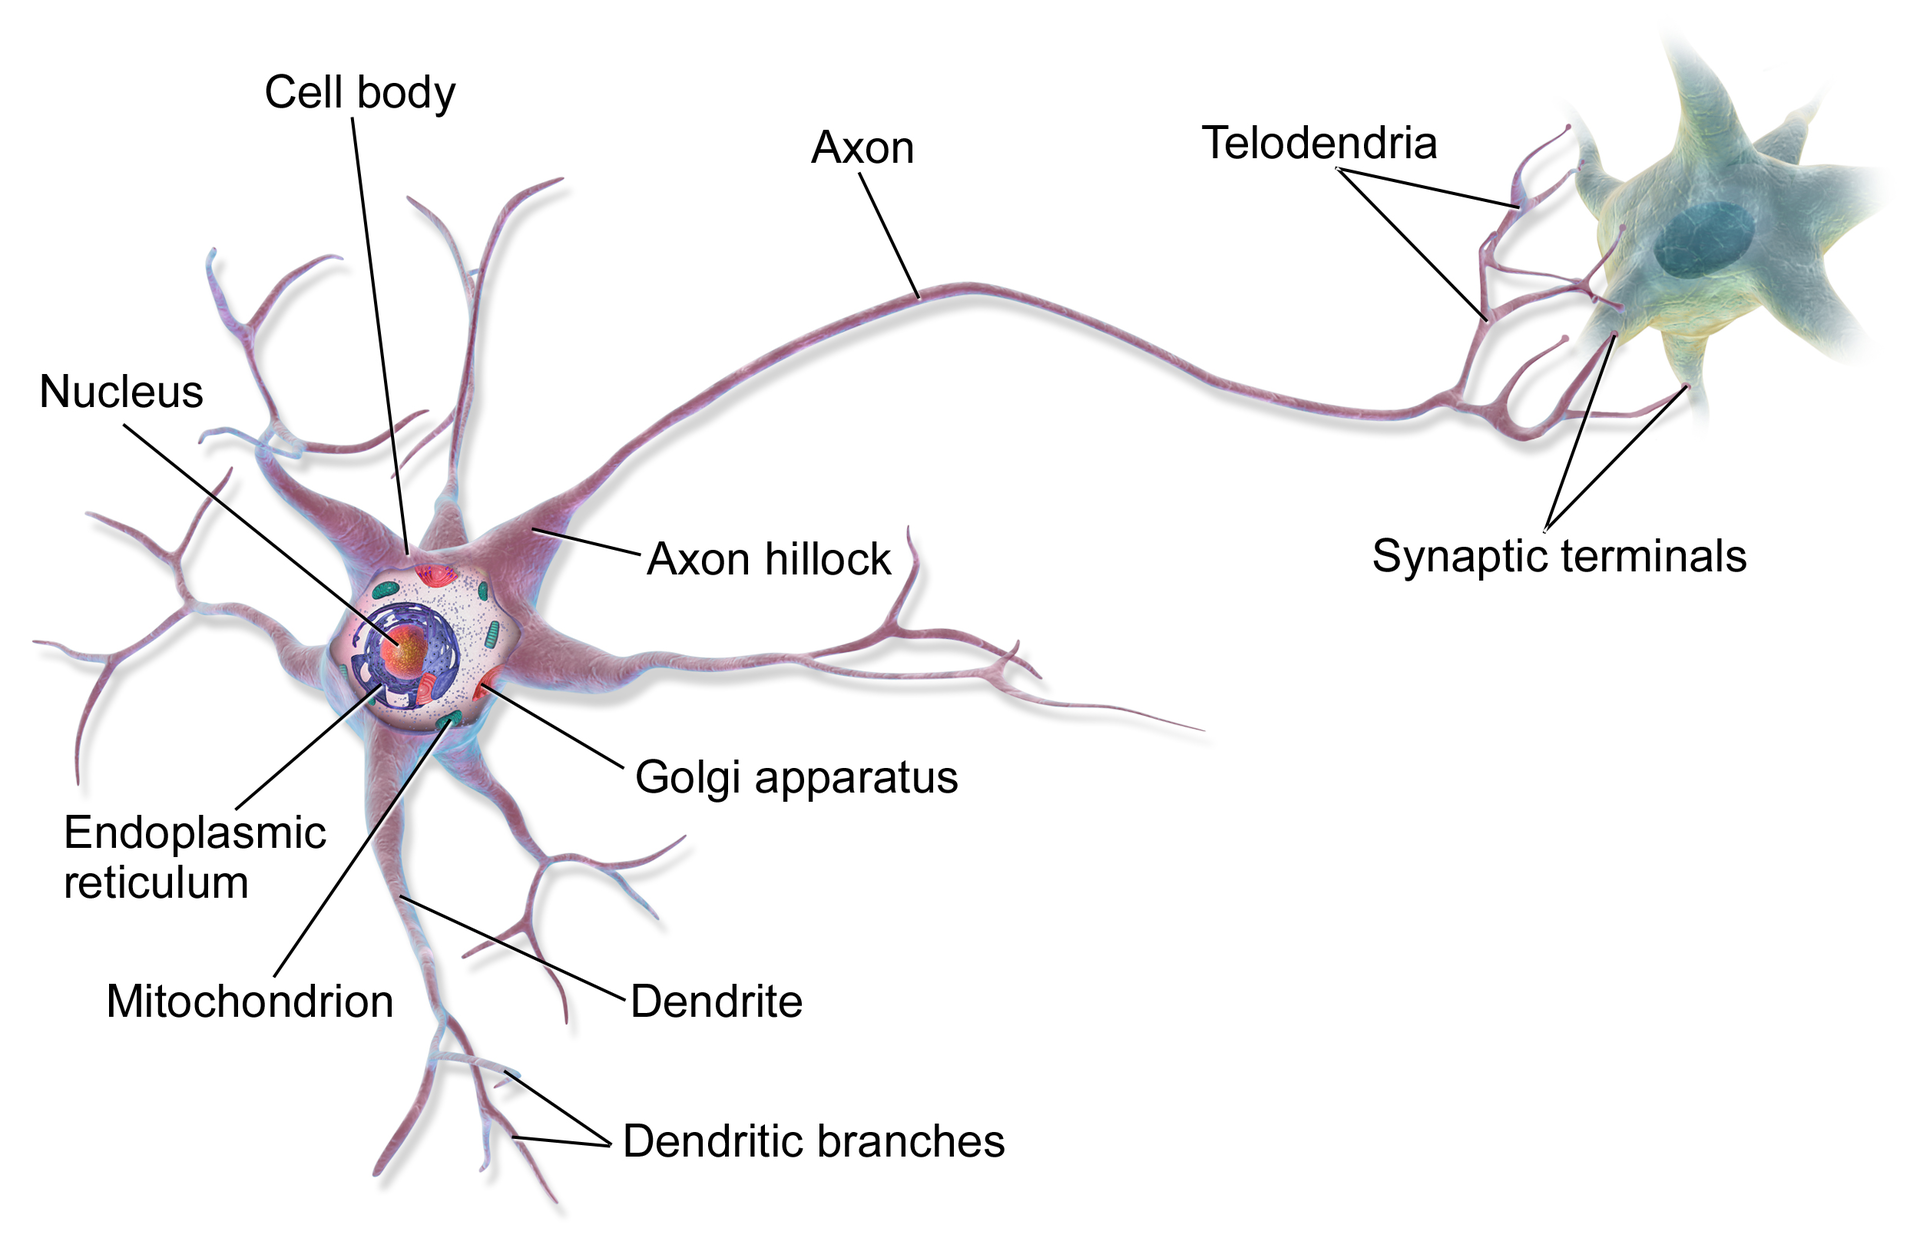
\includegraphics[width=0.5\textwidth]{neuron.png}
\caption{\label{fig:neuron}An example of a neuron taken from wikipedia.}
\end{figure}


Aside from the neuron, other components that make up the neural network model are the \textbf{layers}, a \textbf{loss function} as well as a hyperparameters \textbf{learning rate} and \textbf{momentum}. A \textbf{layer} is a collection of neurons that are related at some point of the decision making process. There are typically 3 layers in a neural network - \textbf{input layer}, \textbf{hidden layer/s} and \textbf{output layer}.

\subsection{Input Layer}
The input layer contains neurons that represent the input values or what the network initially receives from the real world. These values are features that represent a classification/label that we'd like to recognize. In the mathematical model $f(x) = y$, this would be the $x$ as an $n$-dimensional vector. For example, if we'd like to tell the neural network that we're looking at an image of a face represented by a matrix of pixel values, and suppose the size of the image is 32 x 32 pixels, the input layer would have a total of $1024$ neurons each one corresponding to a pixel value. 

\subsection{Hidden Layer/s}
A hidden layer in a neural network contains neurons that processes signals from an adjacent layer (either layer to the left or layer to the right of a hidden layer). A neural network can have more than one hidden layers. For the examples presented in this paper, we will be representing neurons in the hidden layer as $z_{i}$ which we refer to as \textbf{latent variables}. Each of these values receives 

\subsection{Output Layer}
The output layer contains neurons that represent the output of the network or the result/reaction of the network after receiving and processing the input (from input layer to hidden layer then finally to the output layer). The easiest way to model neurons in the output layer is to treat each one (neuron) as a classification/label that the network is trying to recognize with a value ranging from $0$ to $1$. The closer the value to $1$ for an output neuron, the closer it is to thinking that it is that classification or label for a given input $x$. For example, let's say we're trying to learn how to diffirentiate cats from dogs from any other animal. The set of possible outputs (cat, dog or others) can be represented by:

\begin{equation}
  Y=\begin{bmatrix}
    y_{1} &   y_{2} & y_{3}
  \end{bmatrix}
\end{equation}

where $y_{1}$ represents the label cat, $y_{2}$ dog and $y_{3}$ others. A cat then for a neural network would look like $f(x) = \begin{bmatrix} 1 &   0 & 0 \end{bmatrix}$, a dog would be $f(x) = \begin{bmatrix} 0 &  1 & 0 \end{bmatrix}$ and finally any other animal $f(x) = \begin{bmatrix} 0 & 0 & 1 \end{bmatrix}$.

\section{Some examples to get started}

\[ \left( \begin{array}{cc}
1 & 0 \\
0 & 1
\end{array} \right)^{T}
%
=
\left( \begin{array}{cc}
1 & 0 \\
0 & 1
\end{array} \right)
\]

\subsection{How to add Comments}

Comments can be added to your project by clicking on the comment icon in the toolbar above. % * <john.hammersley@gmail.com> 2016-07-03T09:54:16.211Z:
%
% Here's an example comment!
%
To reply to a comment, simply click the reply button in the lower right corner of the comment, and you can close them when you're done.

Comments can also be added to the margins of the compiled PDF using the todo command\todo{Here's a comment in the margin!}, as shown in the example on the right. You can also add inline comments:

\todo[inline, color=green!40]{This is an inline comment.}

\subsection{How to write Mathematics}

\LaTeX{} is great at typesetting mathematics. Let $X_1, X_2, \ldots, X_n$ be a sequence of independent and identically distributed random variables with $\text{E}[X_i] = \mu$ and $\text{Var}[X_i] = \sigma^2 < \infty$, and let
\[S_n = \frac{X_1 + X_2 + \cdots + X_n}{n}
      = \frac{1}{n}\sum_{i}^{n} X_i\]
denote their mean. Then as $n$ approaches infinity, the random variables $\sqrt{n}(S_n - \mu)$ converge in distribution to a normal $\mathcal{N}(0, \sigma^2)$.


\subsection{How to create Sections and Subsections}

Use section and subsections to organize your document. Simply use the section and subsection buttons in the toolbar to create them, and we'll handle all the formatting and numbering automatically.

\subsection{How to add Lists}

You can make lists with automatic numbering \dots

\begin{enumerate}
\item Like this,
\item and like this.
\end{enumerate}
\dots or bullet points \dots
\begin{itemize}
\item Like this,
\item and like this.
\end{itemize}

\subsection{How to add Citations and a References List}

You can upload a \verb|.bib| file containing your BibTeX entries, created with JabRef; or import your \href{https://www.overleaf.com/blog/184}{Mendeley}, CiteULike or Zotero library as a \verb|.bib| file. You can then cite entries from it, like this: \cite{greenwade93}. Just remember to specify a bibliography style, as well as the filename of the \verb|.bib|.

You can find a \href{https://www.overleaf.com/help/97-how-to-include-a-bibliography-using-bibtex}{video tutorial here} to learn more about BibTeX.

We hope you find Overleaf useful, and please let us know if you have any feedback using the help menu above --- or use the contact form at \url{https://www.overleaf.com/contact}!

\bibliographystyle{alpha}
\bibliography{sample}

\end{document}
